\documentclass[tikz,border=0pt]{standalone}
\usepackage[T1]{fontenc}
\usepackage[utf8]{inputenc}
\usepackage{lmodern}
\usepackage{tikz}
\usetikzlibrary{shapes.geometric,arrows.meta,positioning,backgrounds}

% Canvas: 1410pt x 2250pt (scaled to 141mm x 225mm at 10pt/mm)
% We use cm as unit: 14.1cm x 22.5cm

\definecolor{navydark}{HTML}{0f172a}
\definecolor{navyaccent}{HTML}{1e293b}
\definecolor{textwhite}{HTML}{f8fafc}
\definecolor{amber}{HTML}{fbbf24}
\definecolor{softblue}{HTML}{dbeafe}
\definecolor{strokeblue}{HTML}{60a5fa}
\definecolor{softgreen}{HTML}{d1fae5}
\definecolor{strokegreen}{HTML}{34d399}
\definecolor{softpurple}{HTML}{e9d5ff}
\definecolor{strokepurple}{HTML}{a78bfa}
\definecolor{muted}{HTML}{94a3b8}
\definecolor{darkblue}{HTML}{1e3a5f}
\definecolor{darkgreen}{HTML}{14532d}
\definecolor{darkpurple}{HTML}{3b0764}
\definecolor{mid}{HTML}{334155}

\begin{document}
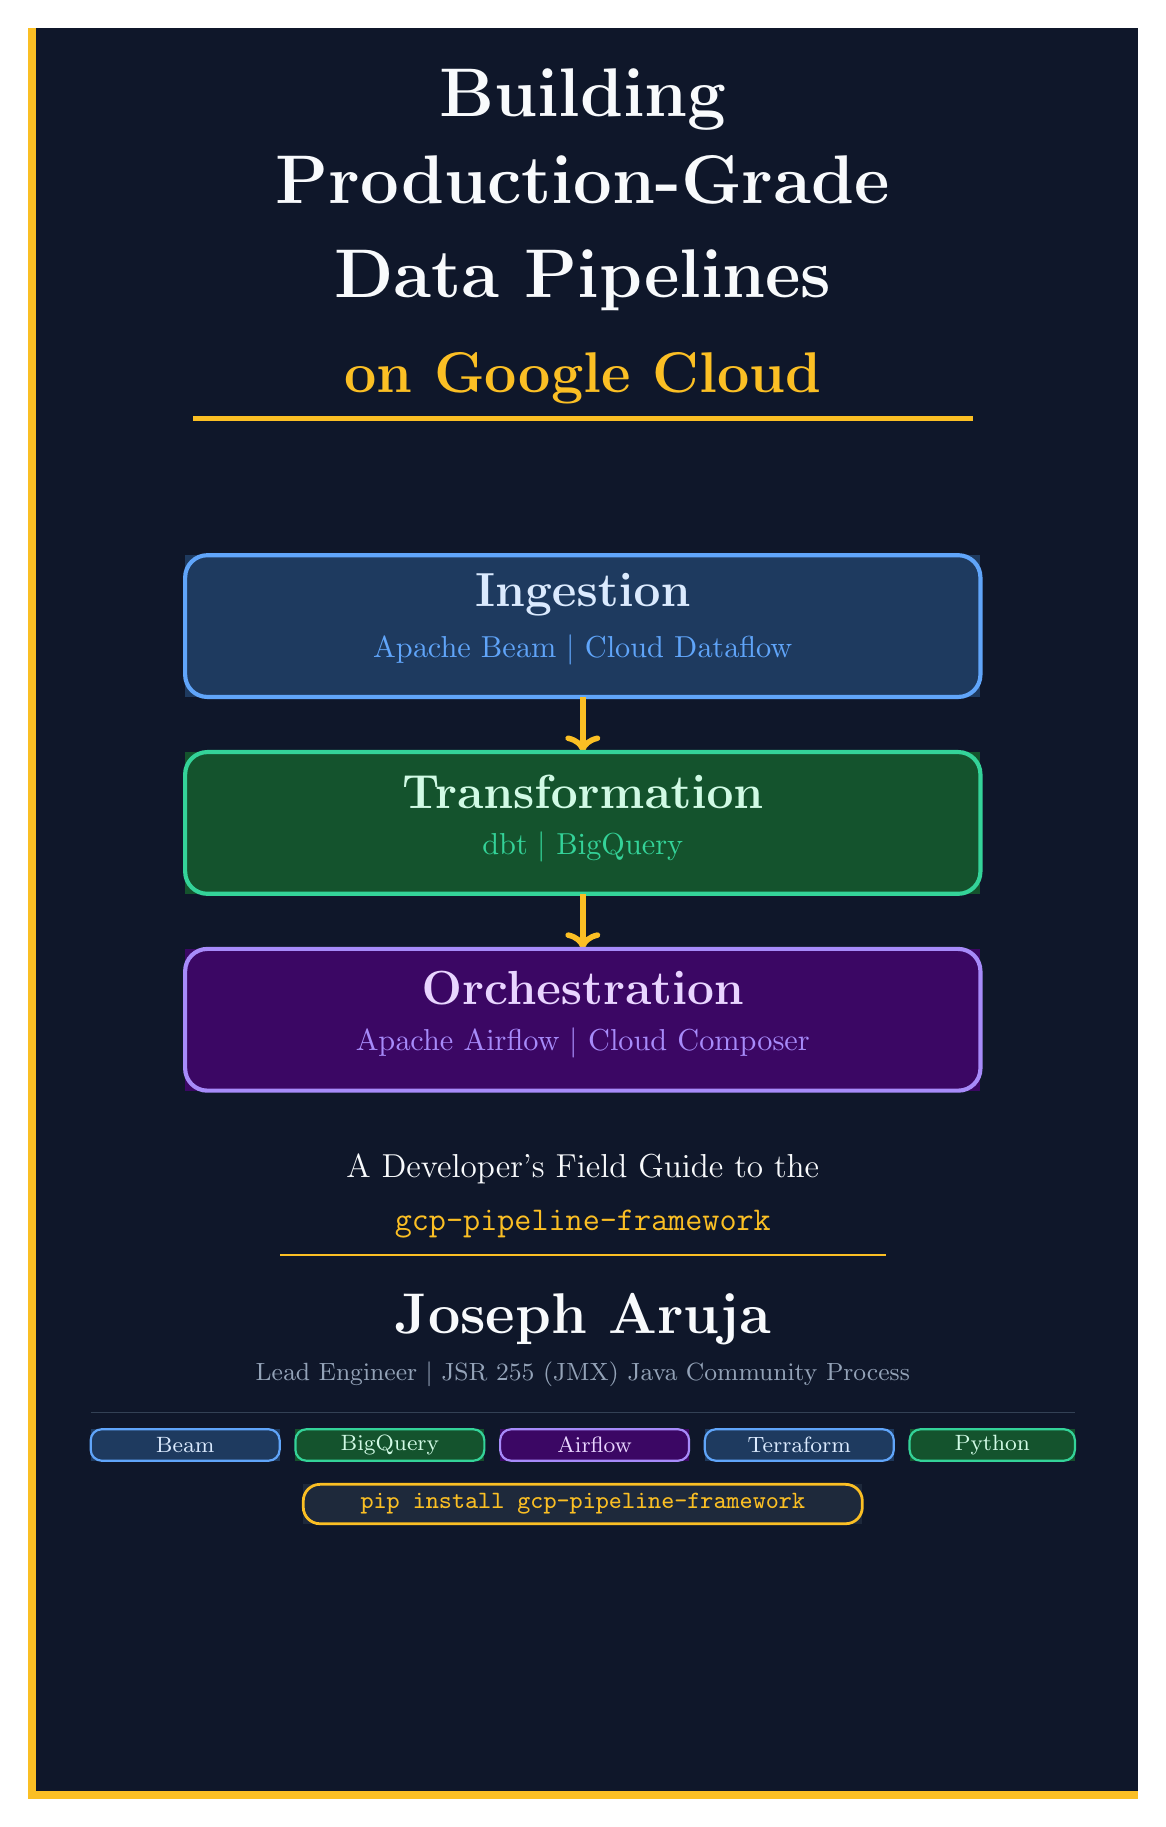
\begin{tikzpicture}[x=1cm,y=1cm]

% Background
\fill[navydark] (0,0) rectangle (14.1,22.5);

% Left accent bar
\fill[amber] (0,0) rectangle (0.1,22.5);

% Bottom accent
\fill[amber] (0,0) rectangle (14.1,0.1);

% ===== TITLE SECTION (top third) =====
\node[anchor=north] at (7.05,22.1)
  {\fontsize{28}{32}\selectfont\bfseries\color{textwhite} Building};
\node[anchor=north] at (7.05,21.0)
  {\fontsize{23}{27}\selectfont\bfseries\color{textwhite} Production-Grade};
\node[anchor=north] at (7.05,19.8)
  {\fontsize{25}{29}\selectfont\bfseries\color{textwhite} Data Pipelines};
\node[anchor=north] at (7.05,18.5)
  {\fontsize{20}{24}\selectfont\bfseries\color{amber} on Google Cloud};

% Amber rule below title
\fill[amber] (2.1,17.5) rectangle (12.0,17.57);

% ===== MIDDLE: THREE-UNIT MODEL =====
% Ingestion box
\fill[darkblue] (2.0,14.0) rectangle (12.1,15.8);
\draw[strokeblue,line width=1.5pt,rounded corners=8pt]
  (2.0,14.0) rectangle (12.1,15.8);
\node[anchor=center] at (7.05,15.3)
  {\fontsize{16}{18}\selectfont\bfseries\color{softblue} Ingestion};
\node[anchor=center] at (7.05,14.6)
  {\fontsize{11}{13}\selectfont\color{strokeblue} Apache Beam \textbar{} Cloud Dataflow};

% Arrow down
\draw[amber,line width=2pt,->] (7.05,14.0) -- (7.05,13.3);

% Transformation box
\fill[darkgreen] (2.0,11.5) rectangle (12.1,13.3);
\draw[strokegreen,line width=1.5pt,rounded corners=8pt]
  (2.0,11.5) rectangle (12.1,13.3);
\node[anchor=center] at (7.05,12.8)
  {\fontsize{16}{18}\selectfont\bfseries\color{softgreen} Transformation};
\node[anchor=center] at (7.05,12.1)
  {\fontsize{11}{13}\selectfont\color{strokegreen} dbt \textbar{} BigQuery};

% Arrow down
\draw[amber,line width=2pt,->] (7.05,11.5) -- (7.05,10.8);

% Orchestration box
\fill[darkpurple] (2.0,9.0) rectangle (12.1,10.8);
\draw[strokepurple,line width=1.5pt,rounded corners=8pt]
  (2.0,9.0) rectangle (12.1,10.8);
\node[anchor=center] at (7.05,10.3)
  {\fontsize{16}{18}\selectfont\bfseries\color{softpurple} Orchestration};
\node[anchor=center] at (7.05,9.6)
  {\fontsize{11}{13}\selectfont\color{strokepurple} Apache Airflow \textbar{} Cloud Composer};

% ===== BOTTOM THIRD =====
% Subtitle
\node[anchor=center] at (7.05,8.0)
  {\fontsize{12}{14}\selectfont\color{textwhite} A Developer's Field Guide to the};
\node[anchor=center] at (7.05,7.3)
  {\fontsize{12}{14}\selectfont\ttfamily\color{amber} gcp-pipeline-framework};

% Small rule
\fill[amber] (3.2,6.9) rectangle (10.9,6.93);

% Author name
\node[anchor=center] at (7.05,6.1)
  {\fontsize{22}{24}\selectfont\bfseries\color{textwhite} Joseph Aruja};

% Author subtitle
\node[anchor=center] at (7.05,5.4)
  {\fontsize{9}{11}\selectfont\color{muted} Lead Engineer \textbar{} JSR 255 (JMX) Java Community Process};

% Bottom rule
\fill[mid] (0.8,4.9) rectangle (13.3,4.92);

% Technology row
\fill[darkblue] (0.8,4.3) rectangle (3.2,4.7);
\draw[strokeblue,line width=0.8pt,rounded corners=4pt] (0.8,4.3) rectangle (3.2,4.7);
\node[anchor=center] at (2.0,4.5)
  {\fontsize{8}{9}\selectfont\color{softblue} Beam};

\fill[darkgreen] (3.4,4.3) rectangle (5.8,4.7);
\draw[strokegreen,line width=0.8pt,rounded corners=4pt] (3.4,4.3) rectangle (5.8,4.7);
\node[anchor=center] at (4.6,4.5)
  {\fontsize{8}{9}\selectfont\color{softgreen} BigQuery};

\fill[darkpurple] (6.0,4.3) rectangle (8.4,4.7);
\draw[strokepurple,line width=0.8pt,rounded corners=4pt] (6.0,4.3) rectangle (8.4,4.7);
\node[anchor=center] at (7.2,4.5)
  {\fontsize{8}{9}\selectfont\color{softpurple} Airflow};

\fill[darkblue] (8.6,4.3) rectangle (11.0,4.7);
\draw[strokeblue,line width=0.8pt,rounded corners=4pt] (8.6,4.3) rectangle (11.0,4.7);
\node[anchor=center] at (9.8,4.5)
  {\fontsize{8}{9}\selectfont\color{softblue} Terraform};

\fill[darkgreen] (11.2,4.3) rectangle (13.3,4.7);
\draw[strokegreen,line width=0.8pt,rounded corners=4pt] (11.2,4.3) rectangle (13.3,4.7);
\node[anchor=center] at (12.25,4.5)
  {\fontsize{8}{9}\selectfont\color{softgreen} Python};

% PyPI badge
\fill[navyaccent] (3.5,3.5) rectangle (10.6,4.0);
\draw[amber,line width=1pt,rounded corners=6pt] (3.5,3.5) rectangle (10.6,4.0);
\node[anchor=center] at (7.05,3.75)
  {\fontsize{9}{11}\selectfont\ttfamily\color{amber} pip install gcp-pipeline-framework};

\end{tikzpicture}
\end{document}
